\providecommand{\main}{..}

\documentclass[\main/main]{subfiles}

\setcounter{chapter}{2} % one before

\begin{document}

\tableofcontents

\chapter[LQR]{Linear Quadratic Regulators}

Up to this point, we have considered decision problems with finitely many states and actions.
However, in many applications, states and actions may take on continuous values.
For example, consider autonomous driving, controlling a robot's joints, and automated manufacturing.
How can we teach computers to solve these kinds of problems? This is the task of \textbf{continuous control}.

\begin{figure}[h]
    \centering
    \begin{subfigure}[b]{0.45\textwidth}
        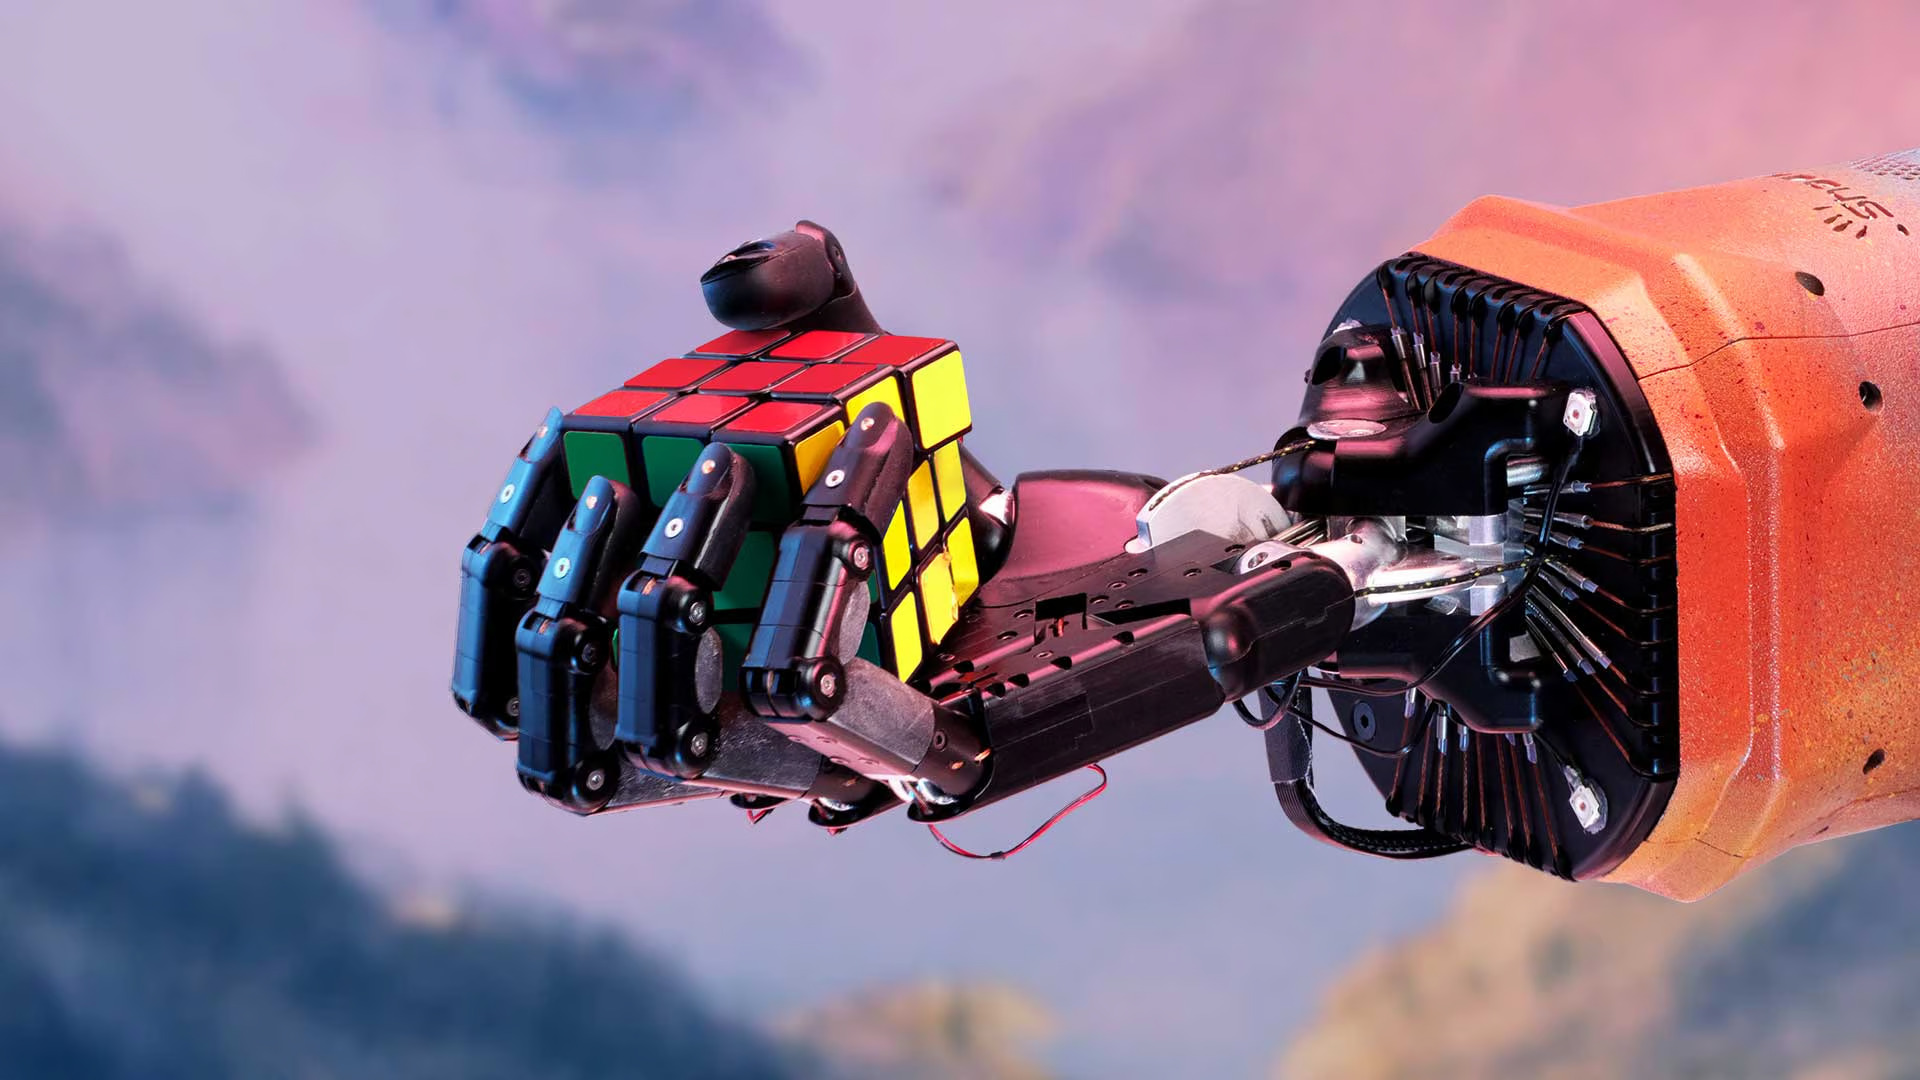
\includegraphics[width=\textwidth]{rubiks_cube.jpg}
        \caption{Solving a Rubik's Cube with a robot hand.}
        \label{fig:rubik\st_cube}
    \end{subfigure}
    \hfill
    \begin{subfigure}[b]{0.45\textwidth}
        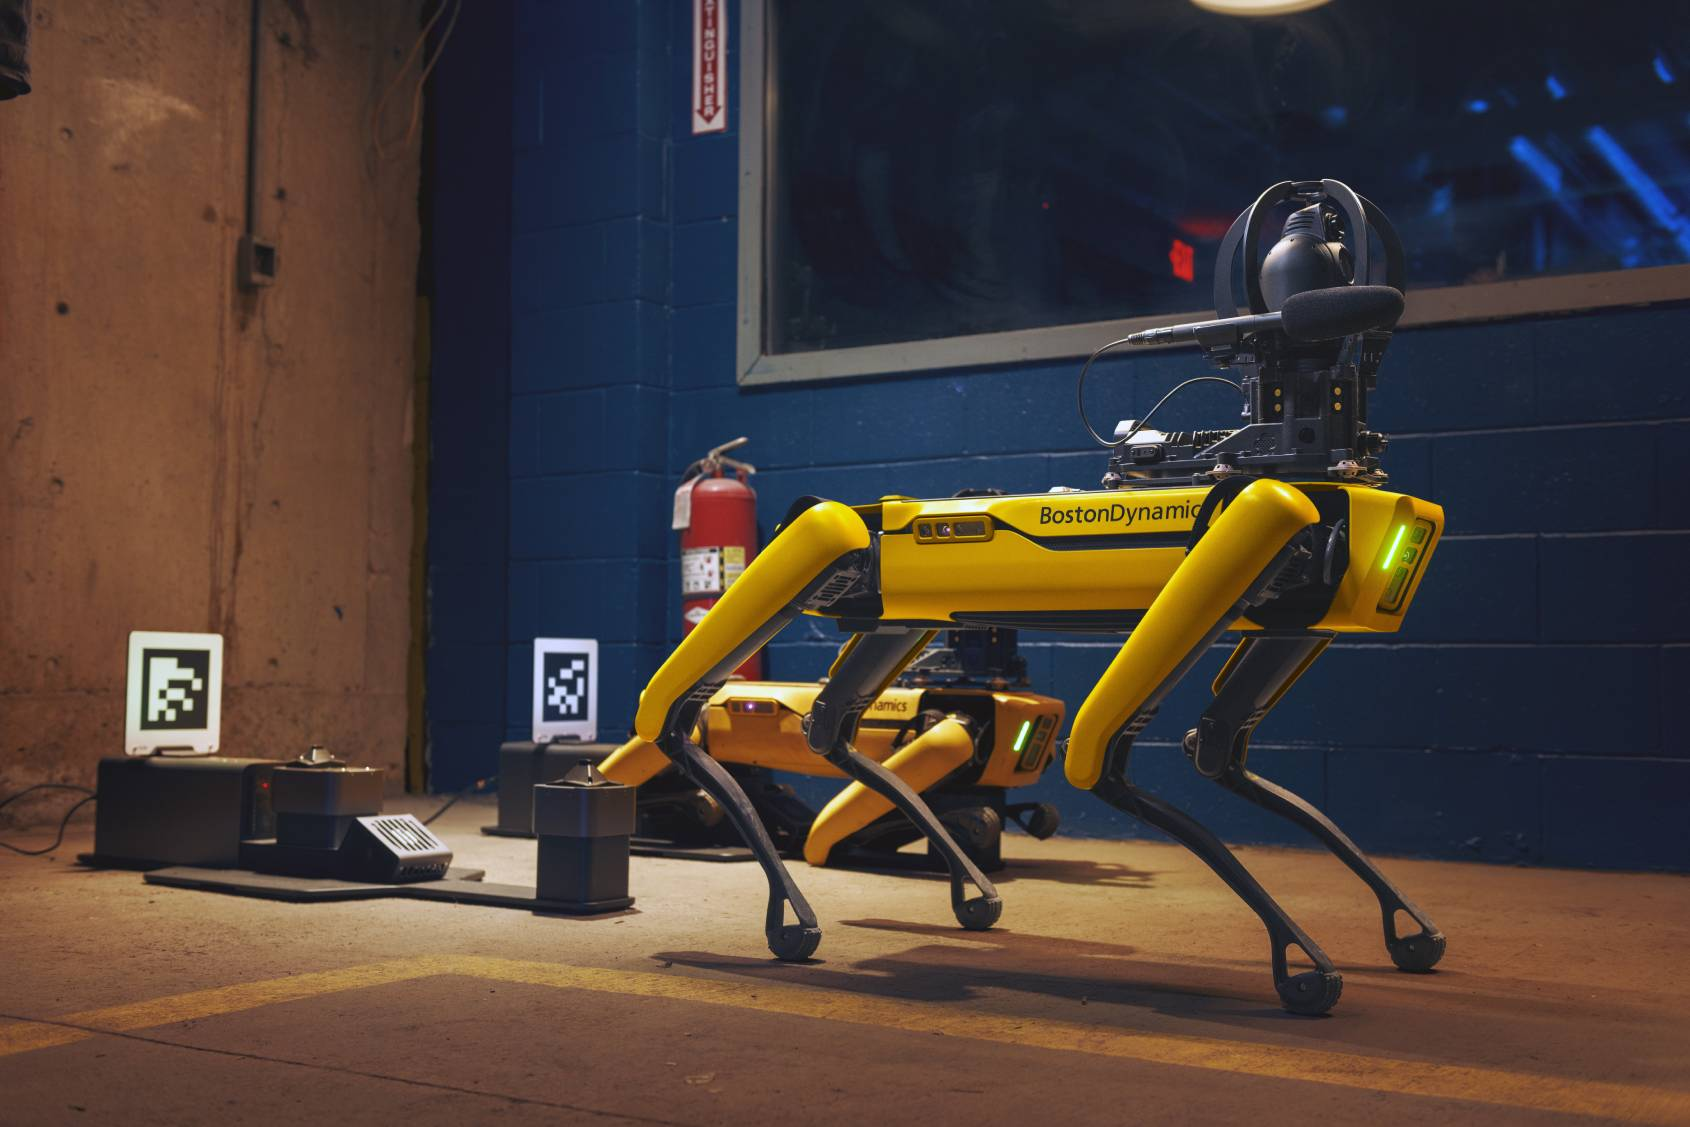
\includegraphics[width=\textwidth]{boston_dynamics.jpg}
        \caption{Boston Dynamics's Spot robot.}
        \label{fig:robot_hand}
    \end{subfigure}
    \caption{Examples of control tasks.}
    \label{fig:control_examples}
\end{figure}

Aside from the change in the state and action spaces, the general problem setup remains the same: we seek to construct an \emph{optimal policy} that outputs actions to solve the desired task. We will see that many key ideas and algorithms, in particular dynamic programming algorithms, carry over to this new setting.

This chapter introduces a fundamental tool to solve a simple class of continuous control problems: the \textbf{linear quadratic regulator}. We will then extend this basic method to more complex settings.


\begin{example}{CartPole}{cart_pole}
    Try to balance a pencil on its point on a flat surface. It's much more difficult than it may first seem: the position of the pencil varies continuously, and the state transitions governing the system, i.e. the laws of physics, are highly complex.
    This task is equivalent to the classic control problem known as \emph{CartPole}:

    \begin{center}
        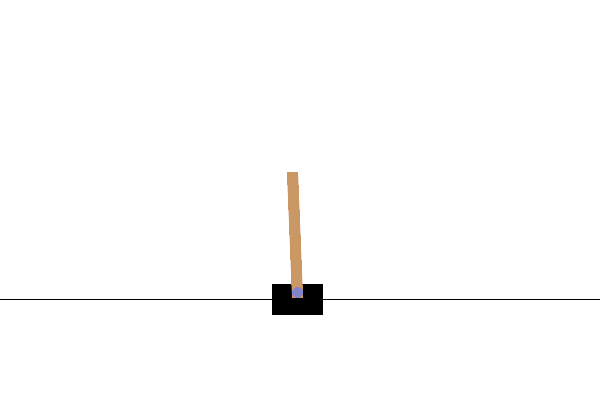
\includegraphics[width=0.4\textwidth]{cart_pole.png}
        % \caption{CartPole: A pole balanced on a cart.}
    \end{center}

    The state $\st \in \R^4$ can be described by:

    \begin{enumerate}
        \item the position of the cart;
        \item the velocity of the cart;
        \item the angle of the pole;
        \item the angular velocity of the pole.
    \end{enumerate}

    We can \emph{control} the cart by applying a horizontal force $\act \in \R$.

    \textbf{Goal:} Stabilize the cart around an ideal state and action $(\st^\star, \act^\star)$.
\end{example}

% In control theory, the state and controls are typically denoted as
% $\st$ and $\act$, but we'll stick with the $\st$ and $\act$ notation to highlight the
% similarity with MDPs.


% Note that we're still assuming that the entire environment is \emph{known} (i.e. the state transitions, rewards, etc). We'll explore the unknown case in the next chapter.

\section{Optimal control}

Recall that an MDP is defined by its state space $\S$, action space $\A$, state transitions $P$, reward function $r$, and discount factor $\gamma$ or time horizon $\hor$. These have equivalents in the control setting:

\begin{itemize}
    \item The state and action spaces are \emph{continuous} rather than finite. That is, $\S \subseteq \R^{n_\st}$ and $\A \subseteq \R^{n_\act}$, where $n_\st$ and $n_\act$ are the corresponding dimensions of these spaces, i.e. the number of coordinates to specify a single state or action respectively.
    \item We call the state transitions the \textbf{dynamics} of the system. In the most general case, these might change across timesteps and also include some stochastic \textbf{noise} $w_\hi$ at each timestep. We denote these dynamics as the function $f_\hi$ such that $\st_{\hi+1} = f_\hi(\st_\hi, \act_\hi, w_\hi)$. Of course, we can simplify to cases where the dynamics are \emph{deterministic/noise-free} (no $w_\hi$ term) and/or \emph{time-homogeneous} (the same function $f$ across timesteps).
    \item Instead of maximizing the reward function, we seek to minimize the \textbf{cost function} $c_\hi: \S \times \A \to \R$. Often, the cost function describes \emph{how far away} we are from a \textbf{target state-action pair} $(\st^\star, \act^\star)$. An important special case is when the cost is \emph{time-homogeneous}; that is, it remains the same function $c$ at each timestep $h$.
    \item We seek to minimize the \emph{undiscounted} cost within a \emph{finite time horizon} $\hor$. Note that we end an episode at the final state $\st_\hor$ -- there is no $\act_\hor$, and so we denote the cost for the final state as $c_\hor(\st_\hor)$.
\end{itemize}

With all of these components, we can now formulate the \textbf{optimal control problem:} \emph{compute a policy to minimize the expected undiscounted cost over $\hor$ timesteps.} In this chapter, we will only consider \emph{deterministic, time-dependent} policies $\pi = (\pi_0, \dots, \pi_{H-1})$ where $\pi_h : \S \to \A$ for each $\hi \in [\hor]$.

\begin{definition}{General optimal control problem}{optimal_control}
    \begin{equation}
        \begin{split}
            \min_{\pi_0, \dots, \pi_{\hor-1} : \S \to \A} \quad & \E \left[
                \left( \sum_{\hi=0}^{\hor-1} c_\hi(\st_\hi, \act_\hi) \right) + c_\hor(\st_\hor)
                \right] \\
            \text{where} \quad & \st_{\hi+1} = f_\hi(\st_\hi, \act_\hi, w_\hi), \\
            & \act_\hi = \pi_\hi(\st_\hi) \\
            & \st_0 \sim \mu_0 \\
            & w_\hi \sim \text{noise}
        \end{split}
    \end{equation}
\end{definition}

% Note that this is a pretty hard problem the way it's written right now!
% We have some pretty strict constraints in the form of the state transitions.

\subsection{A first attempt: Discretization}

Can we solve this problem using tools from the finite MDP setting?
If $\S$ and $\A$ were finite, then we'd be able to work backwards using
the DP algorithm for computing the optimal policy in an MDP \eqref{df:pi_star_dp}.
% In this case, you can also think of $f_\hi$ as an (uncountably infinite-dimensional matrix.
This inspires us to try \emph{discretizing} the problem.

Suppose $\S$ and $\A$ are bounded, that is, $\max_{\st \in \S} \|\st\| \le B_\st$ and
$\max_{\act \in \A} \|\act\| \le B_\act$.
To make $\S$ and $\A$ finite, let's choose some small positive $\epsilon$,
and simply round each coordinate to the nearest multiple of
$\epsilon$. For example, if $\epsilon = 0.01$, then we round each element of $\st$ and $\act$ to two decimal spaces.
% \footnote{Formally, we can consider an $\epsilon$-net over the original continuous space. Let $V$ be some normed space. A subset $V_\epsilon \subseteq V$ is called an $\epsilon$-net if for all $v \in V$, there exists a $v_\epsilon \in V_\epsilon$ such that $\|v - v_\epsilon\| \le \epsilon$. The rounding example given is technically a $0.005$-net.} If both these state and action spaces can be bounded, then the resulting sets are actually finite, so now we can use our previous tools for MDPs.

% The existing algorithms might take unfeasibly long to complete.
However, the discretized $\tilde \S$ and $\tilde \A$ may be finite, but they may be infeasibly large:
we must divide \emph{each dimension} into intervals of length $\varepsilon$,
resulting in $|\tilde \S| = (B_\st/\varepsilon)^{n_\st}$ and $|\tilde \A| = (B_\act/\varepsilon)^{n_\act}$.
To get a sense of how quickly this grows, consider $\varepsilon = 0.01, n_\st = n_\act = 10$. Then the number of elements in the transition matrix would be $|\tilde \S|^2 |\tilde \A| = (100^{10})^2 (100^{10}) = 10^{60}$! (That's a trillion trillion trillion trillion trillion.)

What properties of the problem could we instead make use of? Note that by discretizing the state and action spaces, we implicitly assumed that rounding each state or action vector by some tiny amount $\varepsilon$
wouldn't change the behavior of the system by much;
namely, that the cost and dynamics were relatively \emph{continuous}.
Can we use this continuous structure in other ways? This leads us to the \textbf{linear quadratic regulator}.

\section{The Linear Quadratic Regulator} \label{sec:lqr}

The optimal control problem \eqref{df:optimal_control} seems highly complex in its general case.
Is there a relevant simplification that we can analyze?

Let us consider \emph{linear dynamics} and an \emph{upward-curved quadratic cost function} (in both arguments). We will also consider a time-homogenous cost function that targets $(s^\star, a^\star) = (0, 0)$. This model is called the \textbf{linear quadratic regulator} (LQR) and is a fundamental tool in control theory. Solving the LQR problem will additionally enable us to \emph{locally approximate} more complex setups using \emph{Taylor approximations}.

\begin{definition}{The linear quadratic regulator}{lqr}
    \textbf{Linear, time-homogeneous dynamics}: \[
        \st_{\hi+1} = f(\st_\hi, \act_\hi, w_\hi) = A \st_\hi + B \act_\hi + w_\hi
    \]

    \noindent \textbf{Upward-curved quadratic, time-homogeneous cost function}:
    % TODO Link to that video in the multivariable calculus series
    % \footnote{For some intuition into this expression, consider the simple case where $\act_\hi$ and $\st_\hi$ are scalars (and so are $Q$ and $R$), so $c(\st_\hi, \act_\hi) = Q \st_\hi^2 + R \act_\hi^2$.
    % If this notation is unfamiliar to you, we recommend \href{https://www.khanacademy.org/math/multivariable-calculus/applications-of-multivariable-derivatives/quadratic-approximations/v/expressing-a-quadratic-form-with-a-matrix}{this tutorial on quadratic forms} from Khan Academy!
    % }
    \[
        c(\st_\hi, \act_\hi) = \begin{cases}
            \st_\hi^\top Q \st_\hi + \act_\hi^\top R \act_\hi & \hi < \hor \\
            \st_\hi^\top Q \st_\hi                            & \hi = \hor
        \end{cases}
    \]
    We require $Q$ and $R$ to both be positive definite matrices so that $c$ has a well-defined unique minimum. We can furthermore assume without loss of generality that they are both symmetric (see exercise below).

    % Intuitively, the cost function punishes states and actions that are far away from the origin (i.e. both the state and action are zero vectors). More generally, we'll want to replace the origin with a \emph{goal} state and action $(\st^\star, \act^\star)$. This can easily be done by replacing $\st_\hi$ with $(\st_\hi - \st^\star)$ and $\act_\hi$ with $(\act_\hi - \act^\star)$ in the expression above.


    \noindent \textbf{Spherical Gaussian noise:} \[ w_\hi \sim \mathcal{N}(0, \sigma^2 I) \quad \forall \hi \in [H] \]

    \noindent This results in the LQR optimization problem:
    \begin{align*}
        \min_{\pi_0, \dots, \pi_{\hor-1} : \S \to \A} \quad & \E \left[ \left( \sum_{\hi=0}^{\hor-1} \st_\hi^\top Q \st_\hi + \act_\hi^\top R \act_\hi \right) + \st_\hor^\top Q \st_\hor \right] \\
        \textrm{where} \quad                                & \st_{\hi+1} = A \st_\hi + B \act_\hi + w_\hi                                                                                        \\
                                                            & \act_\hi = \pi_\hi (\st_\hi)                                                                                                        \\
                                                            & w_\hi \sim \mathcal{N}(0, \sigma^2 I)                                                                                               \\
                                                            & \st_0 \sim \mu_0.
    \end{align*}
\end{definition}

\begin{exercise}
    We've set $Q$ and $R$ to be \emph{symmetric} positive definite (SPD) matrices. Here we'll show that the symmetry condition can be imposed without loss of generality. Show that replacing $Q$ with $(Q + Q^\top) / 2$ (which is symmetric) yields the same cost function.
\end{exercise}

\iffalse
    % TODO We went over this example in lecture, but I'm not sure where in the chapter to put it.
    \begin{example}{Driving down a road}{road_lqr}
        Suppose we're driving down a road. At each time step, we can choose an
        action $\act_\hi$: either we accelerate and apply a force forward ($\act_\hi > 0$),
        or reverse and apply a force backward ($\act_\hi < 0$).
        Suppose we can choose an action every $\delta$ seconds, and that our car
        has mass $m$.

        Recall that Newtonian mechanics says that $\text{force} = \text{mass} \times \text{acceleration}$. We can write the acceleration as the change in velocity
        over time, and write the velocity as the change in position over time:

        \begin{align*}
            \text{acceleration}_\hi & = \frac{v_\hi - v_{\hi-1}}{\delta} \\
            v_\hi                   & = \frac{p_\hi - p_{\hi-1}}{\delta} \\
        \end{align*}

        How should we construct our state? We want to express everything in terms
        of these linear dynamics, and we also want our state to be Markov, so that
        we can apply dynamic programming like before.
        Then if we write our state as consisting of the position and velocity, then
        we can write

        \begin{align*}
            p_{\hi+1} & = p_\hi  + \delta v_\hi             \\
            v_{\hi+1} & = v_\hi + \frac{\delta}{m} \act_\hi
        \end{align*}

        Writing everything out in matrix notation, we get: \[
            \st_{\hi+1} = \begin{bmatrix}
                1 & \delta \\
                0 & 1
            \end{bmatrix} \begin{bmatrix}
                p_\hi \\ v_\hi
            \end{bmatrix}
            +
            \begin{bmatrix}
                0 \\ \frac{\delta}{m}
            \end{bmatrix}
            \act_\hi
        \]
    \end{example}
\fi

It will be helpful to reintroduce the \emph{value function} notation for a policy to denote the average cost it incurs.
These will be instrumental in constructing the optimal policy via \textbf{dynamic programming}.

\begin{definition}{Value functions for LQR}{value_lqr}
    Given a policy $\mathbf{\pi} = (\pi_0, \dots, \pi_{\hor-1})$, we can define its
    value function $V^\pi_\hi : \S \to \R$ at time $\hi \in [\hor]$ as the average \textbf{cost-to-go} incurred by that policy:
    \[
        \begin{split}
            V^\pi_\hi (\st) &= \E \left[ \left( \sum_{i=\hi}^{\hor-1} c(\st_i, \act_i) \right) + c(\st_\hor) \mid \st_\hi = \st,  \act_i = \pi_i(\st_i) \quad \forall \hi \le i < H \right] \\
            &= \E \left[ \left( \sum_{i=\hi}^{\hor-1} \st_i^\top Q \st_i + \act_i^\top R \act_i \right) + \st_\hor^\top Q \st_\hor \mid \st_\hi = \st, \act_i = \pi_i(\st_i) \quad \forall \hi \le i < H \right] \\
        \end{split}
    \]

    The Q-function additionally conditions on the first
    action we take:
    \[
        \begin{split}
            Q^\pi_\hi (\st, \act) &= \E \bigg[ \left( \sum_{i=\hi}^{\hor-1} c(\st_i, \act_i) \right) + c(\st_\hor) \\
                &\qquad\qquad \mid  (\st_\hi, \act_\hi) = (\st, \act), \act_i = \pi_i(\st_i) \quad \forall \hi \le i < H \bigg] \\
            &= \E \bigg[ \left( \sum_{i=\hi}^{\hor-1} \st_i^\top Q \st_i + \act_i^\top R \act_i \right) + \st_\hor^\top Q \st_\hor \\
                &\qquad\qquad \mid (\st_\hi, \act_\hi) = (\st, \act), \act_i = \pi_i(\st_i) \quad \forall \hi \le i < H \bigg] \\
        \end{split}
    \]
\end{definition}


\section{Optimality and the Riccati Equation} \label{sec:optimal_lqr}

In this section, we'll compute the optimal value function $V^\star_h$, Q-function $Q^\star_h$, and policy $\pi^\star_h$ in the LQR setting using \textbf{dynamic programming} in a very similar way to the DP algorithms in the MDP setting \eqref{sec:dp}:
\begin{enumerate}
    \item We'll compute $V_H^\star$ (at the end of the horizon) as our base case.
    \item Then we'll work backwards in time, using $V_{h+1}^\star$ to compute $Q_h^\star$, $\pi_{h}^\star$, and $V_h^\star$.
\end{enumerate}
Along the way, we will prove the striking fact that the solution has very simple structure: $V_h^\star$ and $Q^\star_h$ are \emph{upward-curved quadratics} and $\pi_h^\star$ is \emph{linear}.

\begin{definition}[breakable=false]{Optimal value functions for LQR}{optimal_value_lqr}
    The \textbf{optimal value function} is the one that, at any time and in any state,
    achieves \emph{minimum cost} across \emph{all policies}: \[
        \begin{split}
            V^\star_\hi(\st) &= \min_{\pi_\hi, \dots, \pi_{\hor-1}} V^\pi_\hi(\st) \\
            &= \min_{\pi_{\hi}, \dots, \pi_{\hor-1}} \E \bigg[ \left( \sum_{i=\hi}^{\hor-1} \st_\hi^\top Q \st_\hi + \act_\hi^\top R \act_\hi \right) + \st_\hor^\top Q \st_\hor \\
                &\hspace{8em} \mid \st_\hi = \st, \act_i = \pi_i(\st_i) \quad \forall \hi \le i < H \bigg] \\
        \end{split}
    \]
\end{definition}

\begin{theorem}{Optimal value function in LQR is a upward-curved quadratic}{optimal_value_lqr_quadratic}
    At each timestep $h \in [H]$,
    \[
        V^\star_\hi(\st) = \st^\top P_\hi \st + p_\hi
    \]
    for some symmetric positive definite matrix $P_\hi \in \R^{n_\st \times n_\st}$ and vector $p_\hi \in \R^{n_\st}$.
\end{theorem}

\begin{theorem}{Optimal policy in LQR is linear}{optimal_policy_lqr_linear}
    At each timestep $h \in [H]$,
    \[
        \pi^\star_\hi (\st) = - K_\hi \st
    \]
    for some $K_\hi \in \R^{n_\act \times n_\st}$. (The negative is due to convention.)
\end{theorem}


% How can we define an optimal time-dependent policy in this setting?

% It turns out that the optimal policy is one that is deterministic and \emph{linear} at each time
% step! That is, \[ \pi_\hi^\star (\st_\hi) = - K_\hi \st_\hi. \] We'll prove this more
% formally in \autoref{th:optimal_policy_lqr_linear}. This should remind you somewhat of the way in which the optimal policy in
% the previous MDP setting was stationary and deterministic. In both cases,
% it turns out that the optimal policy has special structure!


\textbf{Base case:} At the final timestep, there are no possible actions to take, and so $V^\star_\hor(\st) = c(\st) = \st^\top Q \st$. Thus $V_\hor^\star(\st) = \st^\top P_\hi \st + p_\hi$ where $P_\hor = Q$ and $p_\hor$ is the zero vector.

\textbf{Inductive hypothesis:} We seek to show that the inductive step holds for both theorems: If $V^\star_{\hi+1}(\st)$ is a upward-curved quadratic, then $V^\star_\hi(\st)$ must also be a upward-curved quadratic, and $\pi^\star_\hi(\st)$ must be linear. We'll break this down into the following steps:
\begin{steps}
    \item Show that $Q^\star_\hi(\st, \act)$ is a upward-curved quadratic (in both $\st$ and $\act$).
    \item Derive the optimal policy $\pi^\star_\hi(\st) = \arg \min_\act Q^\star_\hi(\st, \act)$ and show that it's linear.
    \item Show that $V^\star_\hi(\st)$ is a upward-curved quadratic.
\end{steps}
% TODO refer to (This proof is nearly identical to the MDP setting.)
% This is essentially the same proof that we wrote in the finite-horizon MDP setting,
% except now the state and action are \emph{continuous} instead of finite.

We first assume the inductive hypothesis that our theorems are true at time $\hi+1$. That is,
\[ V^\star_{\hi+1}(\st) = \st^\top P_{\hi+1} \st + p_{\hi+1} \quad \forall \st \in \S. \]

\textbf{Step 1.} We aim to show that $Q^\star_\hi(\st)$ is a upward-curved quadratic.
Recall that the definition of $Q^\star_\hi : \S \times \A \to \R$ is \[
    Q^\star_\hi(\st, \act) = c(\st, \act) + \E_{\st' \sim f(\st, \act, w_{\hi+1})} [V^\star_{\hi+1}(\st')].
\]
Recall $c(\st, \act) = \st^\top Q \st + \act^\top R \act$. Let's consider the average value
over the next timestep. The only randomness in the dynamics comes from the noise
$w_{\hi+1} \sim \cN(0, \sigma^2 I)$, so we can write out this expected value as:
\begin{align*}
            & \E_{\st'} [V^\star_{\hi+1}(\st')]                                                                                                         \\
    {} = {} & \E_{w_{\hi+1}} [V^\star_{\hi+1}(A \st + B \act + w_{\hi+1})]                                             &  & \text{definition of } f     \\
    {} = {} & \E_{w_{\hi+1}} [ (A \st + B \act + w_{\hi+1})^\top P_{\hi+1} (A \st + B \act + w_{\hi+1}) + p_{\hi+1} ]. &  & \text{inductive hypothesis}
\end{align*}
Summing and combining like terms, we get \begin{align*}
    Q^\star_\hi(\st, \act) & = \st^\top Q \st + \act^\top R \act + \E_{w_{\hi+1}} [(A \st + B \act + w_{\hi+1})^\top P_{\hi+1} (A \st + B \act + w_{\hi+1}) + p_{\hi+1}] \\
                           & = \st^\top (Q + A^\top P_{\hi+1} A)\st + \act^\top (R + B^\top P_{\hi+1} B) \act + 2 \st^\top A^\top P_{\hi+1} B \act                       \\
                           & \qquad + \E_{w_{\hi+1}} [w_{\hi+1}^\top P_{\hi+1} w_{\hi+1}] + p_{\hi+1}.
\end{align*}
Note that the terms that are linear in $w_\hi$ have mean zero and vanish.
Now consider the remaining expectation over the noise. By expanding out the product and using linearity of
expectation, we can write this out as \begin{align*}
    \E_{w_{\hi+1}} [w_{\hi+1}^\top P_{\hi+1} w_{\hi+1}] & = \sum_{i=1}^d \sum_{j=1}^d (P_{\hi+1})_{ij} \E_{w_{\hi+1}} [(w_{\hi+1})_i (w_{\hi+1})_j].
\end{align*}
When dealing with these \emph{quadratic forms}, it's often helpful to consider the terms
on the diagonal ($i = j$) separately from those off the diagonal. On the diagonal, the
expectation becomes \[ (P_{\hi+1})_{ii} \E (w_{\hi+1})_i^2 = \sigma^2 (P_{\hi+1})_{ii}. \]
% expectation becomes \[ (P_{\hi+1})_{ii} \E (w_{\hi+1})_i^2 = (P_{\hi+1})_{ii} \var \big((w_{\hi+1})_i \big) = \sigma^2 (P_{\hi+1})_{ii}. \]
Off the diagonal, since the elements of $w_{\hi+1}$ are independent,
the expectation factors, and since each element has mean zero, the term disappears: \[ (P_{\hi+1})_{ij} \E [(w_{\hi+1})_i] \E [(w_{\hi+1})_j] = 0. \]
Thus, the only terms left are the ones on the diagonal, so the sum of these can
be expressed as the trace of $\sigma^2 P_{\hi+1}$: \[
    \E_{w_{\hi+1}} [w_{\hi+1}^\top P_{\hi+1} w_{\hi+1}] = \tr(\sigma^2 P_{\hi+1}).
\]
Substituting this back into the expression for $Q^\star_\hi$, we have:

\begin{equation}
    \boxed{
        \begin{aligned}
            Q^\star_\hi(\st, \act) & = \st^\top (Q + A^\top P_{\hi+1} A) \st + \act^\top (R + B^\top P_{\hi+1} B) \act
            + 2\st^\top A^\top P_{\hi+1} B \act                                                                        \\
                                   & \qquad + \tr(\sigma^2 P_{\hi+1}) + p_{\hi+1}.
        \end{aligned}
    }
    \label{eq:q_star_lqr}
\end{equation}

As we hoped, this expression is quadratic in $\st$ and $\act$.
Furthermore, we'd like to show that it also has \emph{positive curvature} with respect to $\act$ so that its minimum with respect to $\act$ is well-defined.
We can do this by proving that the \textbf{Hessian matrix} of second derivatives is positive definite:
\[ \nabla_{\act \act} Q_\hi^\star(x, u) = R + B^\top P_{\hi+1} B \]
This is fairly straightforward:
recall that in our definition of LQR,
we assumed that $R$ is SPD (see \autoref{df:lqr}).
Also note that since $P_{\hi+1}$ is SPD (by the inductive hypothesis), so too must be $B^\top P_{\hi+1} B$. (If this isn't clear, try proving it as an exercise.)
Since the sum of two SPD matrices is also SPD, we have that $R + B^\top P_{\hi+1} B$ is SPD,
and so $Q^\star_\hi$ is indeed a upward-curved quadratic with respect to $\act$.

\textbf{Step 2.} Now we aim to show that $\pi^\star_\hi$ is linear.
Since $Q^\star_\hi$ is a upward-curved quadratic, finding its minimum over $\act$ is easy:
we simply set the gradient with respect to $\act$ equal to zero and solve for $\act$.
First, we calculate the gradient:
\begin{align*}
    \nabla_\act Q^\star_\hi(\st, \act) & = \nabla_\act [ \act^\top (R + B^\top P_{\hi+1} B) \act + 2 \st^\top A^\top P_{\hi+1} B \act ] \\
                                       & = 2 (R + B^\top P_{\hi+1} B) \act + 2 (\st^\top A^\top P_{\hi+1} B)^\top
\end{align*}
Setting this to zero, we get \begin{align}
    0                  & = (R + B^\top P_{\hi+1} B) \pi^\star_\hi(\st) + B^\top P_{\hi+1} A \st \nonumber \\
    \pi^\star_\hi(\st) & = (R + B^\top P_{\hi+1} B)^{-1} (-B^\top P_{\hi+1} A \st) \nonumber              \\
                       & = - K_\hi \st,
\end{align}
where $K_\hi = (R + B^\top P_{\hi+1} B)^{-1} B^\top P_{\hi+1} A$. Note that this optimal policy doesn't depend on the starting distribution $\mu_0$. It's also fully \textbf{deterministic} and isn't affected by the noise terms $w_0, \dots, w_{\hor-1}$.
% (which also held for our finite-horizon MDP solution)
% (Compare this with the discrete MDP case, where calculating our optimal policy
% required taking an expectation over the state transitions.)

\textbf{Step 3.} To complete our inductive proof, we must show that the
inductive hypothesis is true at time $\hi$; that is, we must prove that
$V^\star_\hi(\st)$ is a upward-curved quadratic.
Using the identity $V^\star_\hi(\st) = Q^\star_\hi(\st, \pi^\star(\st))$, we have: \begin{align*}
    V^\star_\hi(\st) & = Q^\star_\hi(\st, \pi^\star(\st))                                                                \\
                     & = \st^\top (Q + A^\top P_{\hi+1} A) \st + (-K_\hi \st)^\top (R + B^\top P_{\hi+1} B) (-K_\hi \st)
    + 2\st^\top A^\top P_{\hi+1} B (-K_\hi \st)                                                                          \\
                     & \qquad + \tr(\sigma^2 P_{\hi+1}) + p_{\hi+1}
\end{align*}
Note that with respect to $\st$, this is the sum of a quadratic term and a constant,
which is exactly what we were aiming for!
The constant term is clearly $p_\hi = \tr(\sigma^2 P_{\hi+1}) + p_{\hi+1}$.
We can simplify the quadratic term by substituting in $K_\hi$.
Notice that when we do this, the $(R+B^\top P_{\hi+1} B)$ term in
the expression is cancelled out by its inverse, and the remaining terms combine to give the \textbf{Riccati equation}:

\begin{definition}{Riccati equation}{riccati}
    \[
        P_\hi = Q + A^\top P_{\hi+1} A - A^\top P_{\hi+1} B (R + B^\top P_{\hi+1} B)^{-1} B^\top P_{\hi+1} A.
    \]
\end{definition}

There are several nice properties to note about the Riccati equation:
\begin{enumerate}
    \item It's defined \textbf{recursively.} Given the dynamics defined by $A$ and $B$, and the state cost matrix $Q$, we can
          recursively calculate $P_\hi$ across all timesteps starting from $P_\hor = Q$.
    \item $P_\hi$ often appears in calculations surrounding optimality, such as $V^\star_\hi, Q^\star_\hi$, and $\pi^\star_\hi$.
    \item Together with the dynamics given by $A$ and $B$, and the action coefficients $R$, it fully defines the optimal policy.
\end{enumerate}

Now we've shown that $V^\star_\hi(\st) = \st^\top P_\hi \st + p_\hi$, which is a upward-curved quadratic, and this concludes our proof. \qed

In summary, we just demonstrated that at each timestep $\hi \in \hor$, the optimal value function $V^\star_\hi$ and optimal Q-function $Q^\star_\hi$ are both upward-curved quadratics and the optimal policy $\pi^\star_\hi$ is linear.
We also showed that all of these quantities can be calculated using a sequence of symmetric matrices $P_0, \dots, P_H$ that can be defined recursively using the Riccati equation \eqref{df:riccati}.

Before we move on to some extensions of LQR, let's consider how the state at time $\hi$ behaves when we act according to this optimal policy.

\subsection{Expected state at time $\hi$}

How can we compute the expected state at time $\hi$ when acting according to the optimal policy?
Let's first express $\st_\hi$ in a cleaner way in terms of the history. Note that having linear dynamics makes it easy to expand terms backwards in time:
\begin{align*}
    \st_\hi & = A \st_{\hi-1} + B \act_{\hi-1} + w_{\hi-1}                                 \\
            & = A (A\st_{\hi-2} + B \act_{\hi-2} + w_{\hi-2}) + B \act_{\hi-1} + w_{\hi-1} \\
            & = \cdots                                                                     \\
            & = A^\hi \st_0 + \sum_{i=0}^{\hi-1} A^i (B \act_{\hi-i-1} + w_{\hi-i-1}).
\end{align*}

Let's consider the \emph{average state} at this time, given all the past states and actions.
Since we assume that $\E [w_\hi] = 0$ (this is the zero vector in $d$ dimensions),
when we take an expectation, the $w_\hi$ term vanishes due to linearity, and so we're left with \[
    \E [\st_\hi \mid \st_{0:(\hi-1)}, \act_{0:(\hi-1)}] = A^\hi \st_0 + \sum_{i=0}^{\hi-1} A^i B \act_{\hi-i-1}.
\]
If we choose actions according to our optimal policy, this becomes \[
    \E [\st_\hi \mid \st_0, \act_i = - K_i \st_i \quad \forall i \le \hi] = \left( \prod_{i=0}^{\hi-1} (A - B K_i) \right) \st_0.
\]
\textbf{Exercise:} Verify this.

This introdces the quantity $A - B K_i$, which shows up frequently in control theory.
For example, one important question is: will $\st_\hi$ remain bounded,
or will it go to infinity as time goes on?
To answer this, let's imagine for simplicity that these $K_i$s are equal (call this matrix $K$).
Then the expression above becomes $(A-BK)^\hi \st_0$.
Now consider the maximum eigenvalue $\lambda_{\max}$ of $A - BK$.
If $|\lambda_{\max}| > 1$, then there's some nonzero initial state $\bar \st_0$, the corresponding eigenvector, for which \[
    \lim_{\hi \to \infty} (A - BK)^\hi \bar \st_0
    = \lim_{\hi \to \infty} \lambda_{\max}^\hi \bar \st_0
    = \infty.
\]
Otherwise, if $|\lambda_{\max}| < 1$, then it's impossible for your original state to explode as dramatically.

\section{Extensions}

We've now formulated an optimal solution for the time-homogeneous LQR
and computed the expected state under the optimal policy.
However, real world tasks rarely have such simple dynamics, and we may wish to design more complex cost functions.
In this section, we'll consider more general extensions of LQR where some of the assumptions we made above are relaxed.
Specifically, we'll consider:
\begin{enumerate}
    \item \textbf{Time-dependency}, where the dynamics and cost function might change depending on the timestep.
    \item \textbf{General quadratic cost}, where we allow for linear terms and a constant term.
    \item \textbf{Tracking a goal trajectory} rather than aiming for a single goal state-action pair.
\end{enumerate}
Combining these will allow us to use the LQR solution to solve more complex setups by taking \emph{Taylor approximations} of the dynamics and cost functions.

\subsection[Time-dependency]{Time-dependent dynamics and cost function} \label{sec:time_dep_lqr}

So far, we've considered the \emph{time-homogeneous} case,
where the dynamics and cost function stay the same at every timestep.
However, this might not always be the case.
As an example, in many sports, the rules and scoring system might change during an overtime period.
To address these sorts of problems, we can loosen the time-homogeneous restriction, and consider the case where the dynamics and cost function are \emph{time-dependent.}
Our analysis remains almost identical; in fact, we can simply add a time index to the matrices $A$ and $B$ that determine the dynamics and the matrices $Q$ and $R$ that determine the cost.

\begin{exercise}
    Walk through the above derivation to verify this claim.
\end{exercise}

The modified problem is now defined as follows:

\begin{definition}{Time-dependent LQR}{time_dependent_lqr}
    \begin{align*}
        \min_{\pi_{0}, \dots, \pi_{\hor-1}} \quad & \E \left[ \left( \sum_{\hi=0}^{\hor-1} (\st_\hi^\top Q_\hi \st_\hi) + \act_\hi^\top R_\hi \act_\hi \right) + \st_\hor^\top Q_\hor \st_\hor \right] \\
        \textrm{where} \quad                      & \st_{\hi+1} = f_\hi(\st_\hi, \act_\hi, w_\hi) = A_\hi \st_\hi + B_\hi \act_\hi + w_\hi                                                             \\
                                                  & \st_0 \sim \mu_0                                                                                                                                   \\
                                                  & \act_\hi = \pi_\hi (\st_\hi)                                                                                                                       \\
                                                  & w_\hi \sim \mathcal{N}(0, \sigma^2 I).
    \end{align*}
\end{definition}

The derivation of the optimal value functions and the optimal policy remains almost exactly the same,
and we can modify the Riccati equation accordingly:

\begin{definition}{Time-dependent Riccati Equation}{riccati_time_dependent}
    \[
        P_\hi = Q_\hi + A_\hi^\top P_{\hi+1} A_\hi - A_\hi^\top P_{\hi+1} B_\hi (R_\hi + B_\hi^\top P_{\hi+1} B_\hi)^{-1} B_\hi^\top P_{\hi+1} A_\hi.
    \]
    Note that this is just the time-homogeneous Riccati equation (\autoref{df:riccati}),
    but with the
    time index added to each of the relevant matrices.
\end{definition}

Additionally, by allowing the dynamics to vary across time,
we gain the ability to \emph{locally approximate} nonlinear dynamics at each timestep.
We'll discuss this later in the chapter.

\subsection[General quadratic cost]{More general quadratic cost functions}

Our original cost function had only second-order terms with respect to the state and action, incentivizing staying as close as possible to $(\st^\star, \act^\star) = (0, 0)$. We can also consider more general quadratic cost functions that also have first-order terms and a constant term.
Combining this with time-dependent dynamics results in the following expression, where we introduce a new matrix $M_\hi$ for the cross term, linear coefficients $q_\hi$ and $r_\hi$ for the state and action respectively, and a constant term $c_\hi$:
\begin{equation}
    c_\hi(\st_\hi, \act_\hi) = ( \st_\hi^\top Q_\hi \st_\hi + \st_\hi^\top M_\hi \act_\hi + \act_\hi^\top R_\hi \act_\hi ) + (\st_\hi^\top q_\hi + \act_\hi^\top r_\hi) + c_\hi.
    \label{df:general_quadratic_cost}
\end{equation}
Similarly, we can also include a constant term $v_\hi \in \R^{n_\st}$ in the dynamics (note that this is \emph{deterministic} at each timestep, unlike the stochastic noise $w_\hi$):
\[
    \st_{\hi+1} = f_\hi(\st_\hi, \act_\hi, w_\hi) = A_\hi \st_\hi + B_\hi \act_\hi + v_\hi + w_\hi.
\]
\begin{exercise}
    Derive the optimal solution. (You will need to slightly modify the above proof.)
\end{exercise}

\subsection{Tracking a predefined trajectory}

Consider applying LQR to a task like autonomous driving, where the target state-action pair changes over time.
We might want the vehicle to follow a predefined \emph{trajectory} of
states and actions $(\st_\hi^\star, \act_\hi^\star)_{\hi=0}^{\hor-1}$. To express this as a control problem, we'll need a corresponding time-dependent cost function:
\[
    c_\hi(\st_\hi, \act_\hi) = (\st_\hi - \st^\star_\hi)^\top Q (\st_\hi - \st^\star_\hi) + (\act_\hi - \act^\star_\hi)^\top R (\act_\hi - \act^\star_\hi).
\]
Note that this punishes states and actions that are far from the intended trajectory. By expanding out these multiplications, we can see that this is actually a special case of the more general quadratic cost function above (\autoref{df:general_quadratic_cost}): \[
    M_\hi = 0, \qquad q_\hi = -2Q \st^\star_\hi, \qquad r_\hi = -2R \act^\star_\hi, \qquad c_\hi = (\st^\star_\hi)^\top Q (\st^\star_\hi) + (\act^\star_\hi)^\top R (\act^\star_\hi).
\]

% TODO infinite horizon

\iffalse
    \section{The infinite-horizon setting $(*)$}

    Another assumption we've made is that the task has a \emph{finite horizon} $\hor$. How about tasks that might continue indefinitely, where we want to minimize the expected cost over \emph{all future timesteps}? Consider, for example, controlling the long-term value of a financial portfolio, or managing acidity levels in a lake.

    For an intuitive perspective on why this happens, let's suppose you have an upcoming project deadline. When it's still a few months away, you might not pay
    much attention to it, and behave as you normally do. But as the deadline gets closer and closer, suddenly the
    horizon becomes more and more relevant, and you'll spend more time thinking about it.
    The infinite-horizon case is just where the deadline is infinitely far away, so you can just behave ``like normal'' all the time!

    In the previous chapter, we dealt with such \textbf{infinite-horizon} cases by \emph{discounting} future rewards. This time, we'll take a different approach by considering the limit of a \emph{finite}-horizon task as $\hor \to \infty$.
    As it turns out, our derivation is exactly analogous to value iteration for MDPs (\autoref{df:value_iteration_pseudocode})!
    However, here the structure is nice enough that we don't need a discount factor $\gamma$ to deal with limits analytically.
    (Note that we must normalize by $1/\hor$ to keep the total cost bounded.)

    In the discounted case, analogously to taking the limit as $\hor \to \infty$, we consider the limit as the discount factor $\gamma$ approaches $1$. This is because as $\gamma \to 1$, time discounting becomes less and less important -- just like the horizon $\hor$ vanishing into the distance -- and we're left with the undiscounted case. (Note that for the total reward to remain bounded, we must normalize the sum by $1 - \gamma$.) Let's consider value iteration in this setting, which uses the Bellman operator $\mathcal{J}$ to update $V$: \[
        V_{\hi+1}(\st) = \lim_{\gamma \to 1} (\mathcal{J} V_\hi)(\st) = \lim_{\gamma \to 1} \max_a \left( r(\st, \act) + \gamma \E_{\st' \sim P(\st, \act)} V_\hi(\st') \right).
    \]
    This is exactly analogous to the \emph{Riccati equation} \eqref{df:riccati}!
    Instead of thinking of $P_{\hi+1}$ as defining the value function for the \emph{next timestep,} though, we think of it as the \emph{next version} of the value function in an iterative algorithm.
    Then both of these algorithms are doing the same thing:
    iteratively refining the value function by acting greedily with respect to the current iteration.

    By going through the same derivation in \autoref{sec:optimal_lqr}, we'll see that $P_\hi$ (defined recursively by the Riccati equation) converges to a fixed value $P$.


    % TODO finish this up

    \begin{figure}[h]
        \centering
        \renewcommand{\arraystretch}{1.5}
        \begin{tabularx}{\textwidth}{m{1in} | >{\centering\arraybackslash}X | >{\centering\arraybackslash}X}
                                                                            & \textbf{Control}                                                                                     & \textbf{Finite MDP}                                                                                         \\
            \hline
            \textbf{State and action spaces}                                & Continuous                                                                                           & Finite                                                                                                      \\
            \hline
            \textbf{Optimization problem}                                   & Minimize finite-horizon undiscounted cost                                                            & Maximize infinite-horizon discounted reward \emph{or} finite-horizon discounted reward                      \\
            \hline
            \textbf{Approaching the infinite-horizon, undiscounted setting} & $\lim_{\hor \to \infty} \frac{1}{\hor} \E \left( \sum_{\hi=0}^{\hor-1} c(\st_\hi, \act_\hi) \right)$ & $\lim_{\gamma \to 1} (1 - \gamma) \E \sum_{\hi=0}^{\infty} \gamma^\hi r(\st_\hi, \act_\hi)$                 \\
            \hline
            \textbf{Iterative algorithm for optimal value}                  & Riccati equations $P := Q + \act^\top P A - \act^\top P B (R + B^\top P B)^{-1} B^\top P A$          & Value iteration $V(\st) := \max_a \left[ r(\st, \act) + \gamma \E_{\st' \sim P(\st, \act)} V(\st') \right]$
        \end{tabularx}
        \caption{A comparison between the continuous control and finite MDP settings.}
        \label{fig:control_mdp}
    \end{figure}

\fi

\section{Approximating nonlinear dynamics} \label{sec:approx_nonlinear}

The LQR algorithm solves for the optimal policy when the dynamics are \emph{linear} and the cost function is an \emph{upward-curved quadratic}.
However, real settings are rarely this simple!
Let's return to the CartPole example from the start of the chapter (\autoref{eg:cart_pole}).
The dynamics (physics) aren't linear. How can we approximate this by an LQR problem?

Concretely, let's consider a \emph{noise-free} problem since, as we saw, the noise doesn't factor into the optimal policy. Let's assume the dynamics and cost function are stationary, and ignore the terminal state for simplicity:

\begin{definition}{Nonlinear control problem}{nonlinear_control}
    \begin{align*}
        \min_{\pi_0, \dots, \pi_{\hor-1} : \S \to \A} \quad & \E_{\st_0} \left[ \sum_{\hi=0}^{\hor-1} c(\st_\hi, \act_\hi) \right] \\
        \text{where} \quad                                  & \st_{\hi+1} = f(\st_\hi, \act_\hi)                                   \\
                                                            & \act_\hi = \pi_\hi(\st_\hi)                                          \\
                                                            & \st_0 \sim \mu_0                                                     \\
                                                            & c(\st, \act) = d(\st, \st^\star) + d(\act, \act^\star).
    \end{align*}
    Here, $d$ denotes a function that measures the ``distance'' between its two arguments.
\end{definition}

This is now only slightly simplified from the general optimal control problem (see \ref{df:optimal_control}). Here, we don't know an analytical form for the dynamics $f$ or the cost function $c$,
but we assume that we're able to \emph{query/sample/simulate} them to get their values at a given state and action.
To clarify, consider the case where the dynamics are given by real world physics.
We can't (yet) write down an expression for the dynamics that we can differentiate or integrate analytically.
However, we can still \emph{simulate} the dynamics and cost function by running a real-world experiment and measuring the resulting states and costs.
How can we adapt LQR to this more general nonlinear case?

\subsection{Local linearization}

How can we apply LQR when the dynamics are nonlinear or the cost function is more complex?
We'll exploit the useful fact that we can take a function that's \emph{locally continuous} around $(s^\star, a^\star)$ and approximate it nearby with low-order polynomials (i.e. its Taylor approximation).
In particular, as long as the dynamics $f$ are differentiable around $(\st^\star, \act^\star)$ and the cost function $c$ is twice differentiable at $(\st^\star, \act^\star)$, we can take a linear approximation of $f$ and a quadratic approximation of $c$ to bring us back to the regime of LQR.

% TODO add Taylor expansion stuff to appendix
% If you're unfamiliar with Taylor expansions, we recommend taking a calculus course; we'll use them here without much further introduction.
Linearizing the dynamics around $(\st^\star, \act^\star)$ gives:
\begin{gather*}
    f(\st, \act) \approx f(\st^\star, \act^\star) + \nabla_\st f(\st^\star, \act^\star) (\st - \st^\star) + \nabla_\act f(\st^\star, \act^\star) (\act - \act^\star) \\
    (\nabla_\st f(\st, \act))_{ij} = \frac{d f_i(\st, \act)}{d \st_j}, \quad i, j \le n_\st \qquad (\nabla_\act f(\st, \act))_{ij} = \frac{d f_i(\st, \act)}{d \act_j}, \quad i \le n_\st, j \le n_\act
\end{gather*}
and quadratizing the cost function around $(\st^\star, \act^\star)$ gives:
\begin{align*}
    c(\st, \act) & \approx c(\st^\star, \act^\star) \quad \text{constant term}                                                                                      \\
                 & \qquad + \nabla_\st c(\st^\star, \act^\star) (\st - \st^\star) + \nabla_\act c(\st^\star, \act^\star) (a - \act^\star) \quad \text{linear terms} \\
                 & \left. \begin{aligned}
                               & \qquad + \frac{1}{2} (\st - \st^\star)^\top \nabla_{\st \st} c(\st^\star, \act^\star) (\st - \st^\star)       \\
                               & \qquad + \frac{1}{2} (\act - \act^\star)^\top \nabla_{\act \act} c(\st^\star, \act^\star) (\act - \act^\star) \\
                               & \qquad + (\st - \st^\star)^\top \nabla_{\st \act} c(\st^\star, \act^\star) (\act - \act^\star)
                          \end{aligned} \right\} \text{quadratic terms}
\end{align*}
where the gradients and Hessians are defined as
\begin{align*}
    (\nabla_\st c(\st, \act))_{i}         & = \frac{d c(\st, \act)}{d \st_i}, \quad i \le n_\st
                                          & (\nabla_\act c(\st, \act))_{i}                                               & = \frac{d c(\st, \act)}{d \act_i}, \quad i \le n_\act               \\
    (\nabla_{\st \st} c(\st, \act))_{ij}  & = \frac{d^2 c(\st, \act)}{d \st_i d \st_j}, \quad i, j \le n_\st
                                          & (\nabla_{\act \act} c(\st, \act))_{ij}                                       & = \frac{d^2 c(\st, \act)}{d \act_i d \act_j}, \quad i, j \le n_\act \\
    (\nabla_{\st \act} c(\st, \act))_{ij} & = \frac{d^2 c(\st, \act)}{d \st_i d \act_j}. \quad i \le n_\st, j \le n_\act
\end{align*}

\textbf{Exercise:} Note that this cost can be expressed in the general quadratic form seen in \autoref{df:general_quadratic_cost}. Derive the corresponding quantities $Q, R, M, q, r, c$.

\subsection{Finite differencing}

To calculate these gradients and Hessians in practice,
we use a method known as \textbf{finite differencing} for numerically computing derivatives.
Namely, we can simply use the limit definition of the derivative,
and see how the function changes as we add or subtract a tiny $\delta$ to the input.
\[
    \frac{d}{dx} f(x) = \lim_{\delta \to 0} \frac{f(x + \delta) - f(x)}{\delta}
\]
Note that this only requires us to be able to \emph{query} the function, not to have an analytical expression for it,
which is why it's so useful in practice.
% TODO Do we need to go further into detail about finite differencing?

\subsection{Local convexification}

However, simply taking the second-order approximation of the cost function is insufficient,
since for the LQR setup we required that the $Q$ and $R$ matrices were positive definite, i.e. that all of their eigenvalues were positive.

One way to naively \emph{force} some symmetric matrix $D$ to be positive definite is to set any non-positive eigenvalues to some small positive value $\varepsilon > 0$.
Recall that any real symmetric matrix $D \in \R^{n \times n}$ has an basis of eigenvectors $u_1, \dots, u_n$ with corresponding eigenvalues $\lambda_1, \dots, \lambda_n$ such that $D u_i = \lambda_i u_i$. Then we can construct the positive definite approximation by \[
    \widetilde{D} = \left( \sum_{i=1, \dots, n \mid \lambda_i > 0} \lambda_i u_i u_i^\top \right) + \varepsilon I.
\]

\textbf{Exercise:} Convince yourself that $\widetilde{D}$ is indeed positive definite.

Note that Hessian matrices are generally symmetric, so we can apply this process to $Q$ and $R$ to obtain the positive definite approximations $\widetilde{Q}$ and $\widetilde{R}$. Now that we have a upward-curved quadratic approximation to the cost function, and a linear approximation to the state transitions, we can simply apply the time-homogenous LQR methods from \autoref{sec:optimal_lqr}.

% TODO: insert figure here for visual intuition, in case people aren't experienced with the calculus

But what happens when we enter states far away from $\st^\star$ or want to use actions far from $\act^\star$?
A Taylor approximation is only accurate in a \emph{local} region around the point of linearization,
so the performance of our LQR controller will degrade as we move further away.
We'll see how to address this in the next section using the \textbf{iterative LQR} algorithm.
\begin{figure}[h]
    \centering
    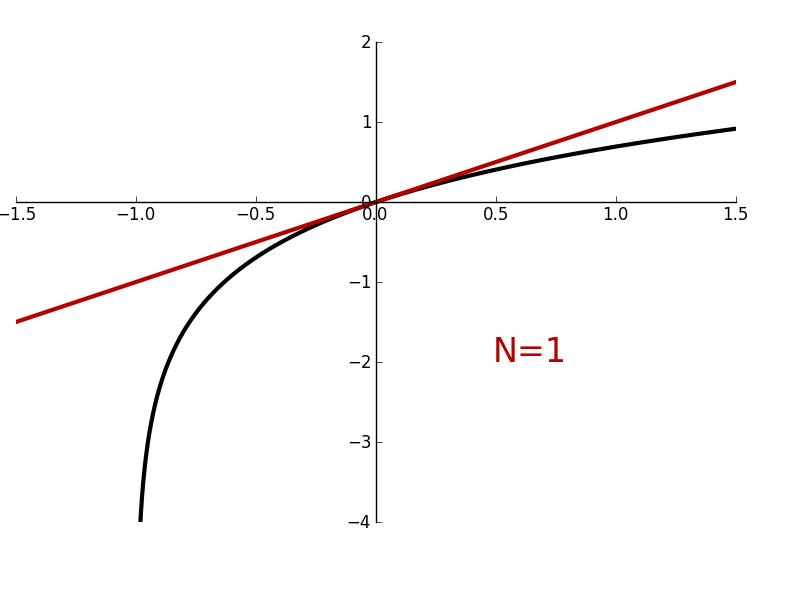
\includegraphics[width=0.5\textwidth]{log_taylor.png}
    \caption{Local linearization might only be accurate in a small region around the point of linearization.}
    \label{fig:local_linearization}
    % https://upload.wikimedia.org/wikipedia/commons/2/27/Logarithm_GIF.gif
\end{figure}

\subsection{Iterative LQR}

To address these issues with local linearization, we'll use an iterative approach, where we repeatedly linearize around different points to create a \emph{time-dependent} approximation of the dynamics, and then solve the resulting time-dependent LQR problem to obtain a better policy.
This is known as \textbf{iterative LQR} or \textbf{iLQR}:

\begin{definition}{Iterative LQR (high-level)}{ilqr}
    For each iteration of the algorithm:
    \begin{steps}
        \item Form a time-dependent LQR problem around the current candidate trajectory using local linearization.
        \item Compute the optimal policy using \autoref{sec:time_dep_lqr}.
        \item Generate a new series of actions using this policy.
        \item Compute a better candidate trajectory by interpolating between the current and proposed actions.
    \end{steps}
\end{definition}

Now let's go through the details of each step. We'll use superscripts to denote the iteration of the algorithm. We'll also denote $\bar \st_0 = \E_{\st_0 \sim \mu_0} [\st_0]$ as the expected initial state.

At iteration $i$ of the algorithm, we begin with a \textbf{candidate} trajectory $\bar \tau^i = (\bar \st^i_0, \bar \act^i_0, \dots, \bar \st^i_{\hor-1}, \bar \act^i_{\hor-1})$.

\textbf{Step 1: Form a time-dependent LQR problem.}
At each timestep $\hi \in [\hor]$, we use the techniques from \autoref{sec:approx_nonlinear} to linearize the dynamics and quadratize the cost function around $(\bar \st^i_\hi, \bar \act^i_\hi)$:
\begingroup
\newcommand{\iter}[1]{\bar {#1}^i_\hi}
\newcommand{\grad}[2]{\nabla_{#2} #1(\iter \st, \iter \act)}
\begin{align*}
    f_\hi(\st, \act) & \approx f(\iter \st, \iter \act) + \grad f \st (\st - \iter \st) + \grad f \act (\act - \iter \act)                         \\
    c_\hi(\st, \act) & \approx c(\iter \st, \iter \act) + \begin{bmatrix}
                                                              \st - \iter \st & \act - \iter \act
                                                          \end{bmatrix} \begin{bmatrix}
                                                                            \grad c \st \\
                                                                            \grad c \act
                                                                        \end{bmatrix}                                                      \\
                     & \qquad + \frac{1}{2} \begin{bmatrix}
                                                \st - \iter \st & \act - \iter \act
                                            \end{bmatrix} \begin{bmatrix}
                                                              \nabla_{\st \st} c(\iter \st, \iter \act)  & \nabla_{\st \act} c(\iter \st, \iter \act)  \\
                                                              \nabla_{\act \st} c(\iter \st, \iter \act) & \nabla_{\act \act} c(\iter \st, \iter \act)
                                                          \end{bmatrix}
    \begin{bmatrix}
        \st - \iter \st \\
        \act - \iter \act
    \end{bmatrix}.
\end{align*}
\endgroup

\textbf{Step 2: Compute the optimal policy.}
We can now solve the time-dependent LQR problem using the Riccati equation from \autoref{sec:time_dep_lqr} to compute the optimal policy $\pi^i_0, \dots, \pi^i_{\hor-1}$.

\textbf{Step 3: Generate a new series of actions.}
We can then generate a new sample trajectory by taking actions according to this optimal policy: \[
    \bar \st^{i+1}_0 = \bar \st_0, \qquad \tilde \act_\hi = \pi^i_\hi(\bar \st^{i+1}_\hi), \qquad \bar \st^{i+1}_{\hi+1} = f(\bar \st^{i+1}_\hi, \tilde \act_\hi).
\]
Note that the states are sampled according to the \emph{true} dynamics, which we assume we have query access to.

\textbf{Step 4: Compute a better candidate trajectory.},
Note that we've denoted these actions as $\tilde \act_\hi$ and aren't directly using them for the next iteration $\bar \act^{i+1}_\hi$.
Rather, we want to \emph{interpolate} between them and the actions from the previous iteration $\bar \act^i_0, \dots, \bar \act^i_{\hor-1}$.
This is so that the cost will \emph{increase monotonically,} since if the new policy turns out to actually be worse, we can stay closer to the previous trajectory. (Can you think of an intuitive example where this might happen?)

Formally, we want to find $\alpha \in [0, 1]$ to generate the next iteration of actions $\bar \act^{i+1}_0, \dots, \bar \act^{i+1}_{\hor-1}$ such that the cost is minimized:
\begin{align*}
    \min_{\alpha \in [0, 1]} \quad & \sum_{\hi=0}^{\hor-1} c(\st_\hi, \bar \act^{i+1}_\hi)                     \\
    \text{where} \quad             & \st_{\hi+1} = f(\st_\hi, \bar \act^{i+1}_\hi)                             \\
                                   & \bar \act^{i+1}_\hi = \alpha \bar \act^i_\hi + (1-\alpha) \tilde \act_\hi \\
                                   & \st_0 = \bar \st_0.
\end{align*}
Note that this optimizes over the closed interval $[0, 1]$, so by the Extreme Value Theorem, it's guaranteed to have a global maximum.

The final output of this algorithm is a policy $\pi^{n_\text{steps}}$ derived after $n_\text{steps}$ of the algorithm.
Though the proof is somewhat complex, one can show that for many nonlinear control problems, this solution converges to a locally optimal solution (in the policy space).

% TODO programming
\iffalse
    \section{Programming and Implementation}

    Not sure how much to include here yet. WIP. Walk through a basic Python solution
    to OpenAI Gym and CartPole? (Or save this for homework?)
\fi

\iffalse
    \section{Exercises}

    \begin{enumerate}
        \item Consider a cleaning robot with one wheel on each side of its body. Your pet has made a mess nearby, and you want to steer the robot to go clean it up.
              Let's represent the state of the robot as a $3$-dimensional vector containing its $(x, y)$ coordinates and its angle $\theta$, relative to some global reference frame.
              We can control the robot using its linear velocity $v$ (change in $x, y$) and angular velocity $\omega$ (change in $\theta$).
              For simplicity, we'll assume the robot is perfectly ideal and there's no noise in the system.
              \begin{enumerate}
                  \item Formally describe the true of the system as a function $f : \S \times \A \to \S$. Assume the system works in timesteps of $dt = 1 \st$ and that all distances are measured in meters.
                  \item Linearize the dynamics that you derived using a first-order Taylor approximation. Is this approximation stationary or time-dependent?
                  \item Suppose the mess is at location $(x^\star, y^\star) = (2, 2)$. We want to reach that state using a small amount of energy. Write down the quadratic cost function using $Q = \diag(1, 1, 0.5)$, expressing that we care about the final position more than the state, and $R = 0.2 I$ to penalize large action steps.
              \end{enumerate}
              Now that our LQR is set up, let's find the optimal policy.
              \begin{enumerate}
                  \item Let the horizon be $\hor = 50$ timesteps. Write down the recursive update formula for $P_\hi$ (Hint: use the Riccati equation).
                  \item Write the closed form solution of the optimal policy at time $\hor-1$. Verify that this is a linear function of the state.
              \end{enumerate}

        \item (Todo.)


    \end{enumerate}

\fi

\section{Summary}

This chapter introduced some approaches to solving different variants of the optimal control problem \eqref{df:optimal_control}.
We began with the simple case of linear dynamics and an upward-curved quadratic cost. This model is called the LQR and we solved for the optimal policy using dynamic programming. We then extended these results to the more general nonlinear case via local linearization. We finally saw the iterative LQR algorithm for solving nonlinear control problems.

\end{document}


